\documentclass[
    a4paper,
    twocolumn,
]{article}

% Table insertions
% --------------------------------------------------
\usepackage{graphics}

% Image insertions
% --------------------------------------------------
\usepackage{graphicx}
\usepackage[belowskip=-3pt,aboveskip=8pt]{caption}
\graphicspath{{./images/}}

% Input and font encoding
% --------------------------------------------------
\usepackage[utf8]{inputenc}
\usepackage[T1]{fontenc}

% biblatex --- Bibliography setup
% --------------------------------------------------
\usepackage[
    backend=biber,
    style=numeric,
    sorting=none,
]{biblatex}

\addbibresource{sources.bib}

% hyperref --- Hyperlinks in PDF
% --------------------------------------------------
\usepackage[pdfusetitle]{hyperref}

% Set colors of links
\hypersetup{
    colorlinks=true,
    linkcolor=magenta,
    citecolor=,
    urlcolor=blue,
}

% Allow line-breaks in links and URLs
\hypersetup{breaklinks=true}

% Use the normal document font for URLs rather than monospace
\urlstyle{same}

% Document Metadata
% --------------------------------------------------
\title{INF3200: Mandatory Assignment 1}
\author{Yasiru Rathsara Witharanage}
\date{\today}

% Document
% --------------------------------------------------
\begin{document}

\maketitle

\begin{abstract}
    \textbf{In an ever-growing tech-world, the necessity of storing and accessing data is vital. With the expansion of industry and users, data-stores are being required to address additional requirements apart from its main objective, such as scalability, replication, accessibility etc. To this end, distributed data-stores have been more useful and applicable. In this study, I have implemented a distributed hash table using chord~\cite{1} and conducted few experiments to observe how its performance differs with cluster's scale and number of requests in the batch.}
\end{abstract}

\section{Introduction}

The primary objective of this study is to build a system of distributed nodes acting as a single key-value store with the assistance of a distributed hash table 'chord', which uses a ring network of individual nodes with distributed memory each with the knowledge of only a partition of the entire network. This store exposes the following HTTP endpoints for querying and debugging purposes.

\begin{itemize}
	\item PUT /storage/key - to store a value provided in the raw body
	\item GET /storage/key - to retrieve the value of a key (returned in raw body)
	\item GET /neighbors - to retrieve the neighbours of a node
\end{itemize}

\section{Project Description}
\subsection{Design}

Each individual node in the network is given an id based on the SHA256 hash value of its own hostname. Thus, specific instances were chosen to resemble and organize the ring structure such that there are no multiple instances for the same id. Figure.1 shows one of such structures with 16 nodes used in the experiments of this study along with generated node ids and hostnames.

\setlength{\intextsep}{10pt plus 2pt minus 2pt}
\begin{figure}[!ht]
	\centering
	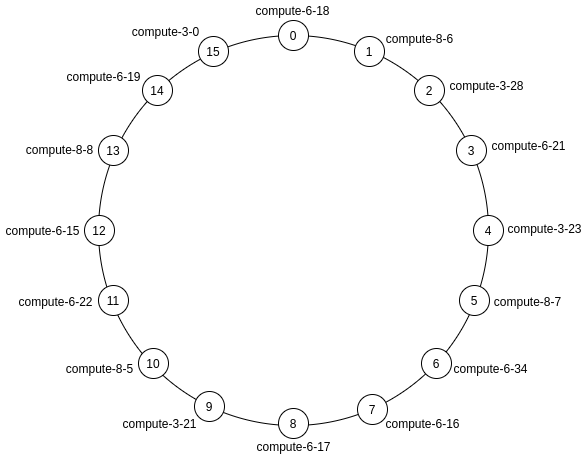
\includegraphics[width=7.5cm]{16-structure.png}
	\caption{Ring structure with 16-nodes}
\end{figure}

Each node is only aware of its neighbours, i.e. predecessor and successor. These values can be configured before the execution of a node. \\

Whenever a query is received by a node, it initially checks whether the requested key belongs to itself and if not, it proceeds to the immediate successor. This process is iterated until the correct node for key is discovered and the corresponding response is returned along the same route. 

\subsection{Implementation}

Golang was used for the implementation of chord with a flat-hierarchical code structure and different layers for each functionality. HTTP endpoints listed previously were implemented in HTTP layer while node layer contains details (node id, predecessor, successor) related with the node along with validating key function. SHA256 was used for hashing of both key and node id to match with relevant buckets. A separate HTTP client was used in neighbour layer to proceed any request with a key that does not belong to the corresponding node. All key-value entry pairs are stored in an in-memory map which is specifically designed for concurrent use.\\

A sample set is given below for the configuration values of parameters required by the implementation but however user is allowed to provide his own desired values for service configurations. Predecessor and successor ports can be given null if they are same as the port of current node.

\begin{verbatim}
	# service configs
	port: 52520
	max_num_of_nodes: 16
	request_timeout_sec: 2
	ttl_min: 180
	
	# neighbour configs
	finger_table_enabled: false
	neighbour_check: false
	predecessor: "compute-1-1"
	predecessor_port: ""
	successor: "compute-1-1"
	successor_port: ""
	
	# logger configs
	colors_enabled: true
	log_level: "TRACE"
	file_path: true
\end{verbatim}

\texttt{max\_num\_of\_nodes} here should be equal or larger than the number of nodes being tested. \texttt{request\_timeout\_sec} refers to the waiting time of a single HTTP request by a node in seconds. Moreover each node has a TTL in minutes for the self-termination configured by \texttt{ttl\_min}.

\section{Evaluation}

Several experiments were carried out to measure and evaluate latency variation under different circumstances. A separate client was implemented for this testing purpose and can be found under tester directory of the project. 

In these experiments, a number of requests was sent and total latency of the whole batch was measured in order to calculate the average latency per request in different scenarios. This entire process was done several times by changing load (number of requests) and number of nodes in the cluster. \\

A set of 15 dummy requests was used in these attempts where each request consists of a key belonging to a separate bucket, thus minimizing the erroneous influence of a particular node on a test attempt. This set was iterated as many times as required until the number of requests being tested was matched.\\

Table 1 and 2 provide details about hardware specifications of nodes and sets of nodes used in each experiment.

\begin{table}[!ht]
\renewcommand{\arraystretch}{1.4}
\centering
\resizebox{\columnwidth}{!}{%
\begin{tabular}{|c | c | c | c | c | c|} 
	\hline
	Node ID & Hostname & Model & CPUs & Cores & Processors\\
	\hline
	0 & compute-6-18 & Lenovo P310 & 1 & 4 & 4 \\ 
	\hline
	1 & compute-8-6 & Lenovo m93p & 1 & 4 & 8 \\ 
	\hline
	2 & compute-3-28 & Dell T3600 & 1 & 4 & 4 \\ 
	\hline
	3 & compute-6-21 & Lenovo P310 & 1 & 4 & 4 \\ 
	\hline
	4 & compute-3-23 & Dell T3600 & 1 & 4 & 4 \\ 
	\hline
	5 & compute-8-7 & Lenovo m93p & 1 & 4 & 8 \\ 
	\hline
	6 & compute-6-34 & Lenovo P310 & 1 & 4 & 4 \\ 
	\hline
	7 & compute-6-16 & Lenovo P310 & 1 & 4 & 4 \\ 
	\hline
	8 & compute-6-17 & Lenovo P310 & 1 & 4 & 4 \\ 
	\hline
	9 & compute-3-21 & Dell T3600 & 1 & 4 & 4 \\ 
	\hline
	10 & compute-8-5 & Lenovo m93p & 1 & 4 & 8 \\ 
	\hline
	11 & compute-6-22 & Lenovo P310 & 1 & 4 & 4 \\ 
	\hline
	12 & compute-6-15 & Lenovo P310 & 1 & 4 & 4 \\ 
	\hline
	13 & compute-8-8 & Lenovo m93p & 1 & 4 & 8 \\ 
	\hline
	14 & compute-6-19 & Lenovo P310 & 1 & 4 & 4 \\ 
	\hline
	15 & compute-3-0 & Dell T3600 & 1 & 4 & 4 \\ 
	\hline
\end{tabular}%
}
\caption{Hardware specification of nodes}
\end{table}

\begin{table}[!ht]
	\renewcommand{\arraystretch}{1.1}
	\centering
	\resizebox{\columnwidth}{!}{%
		\begin{tabular}{|c | l|} 
			\hline
			Number of nodes &\multicolumn{1}{|c|}{Node IDs} \\
			\hline
			1 & 10 \\ 
			\hline
			2 & 0, 7 \\
			\hline
			4 & 2, 5, 8, 11 \\
			\hline
			8 & 0, 1, 4, 6, 8, 9, 10, 13 \\
			\hline
			16 & 0, 1, 2, 3, 4, 5, 6, 7, 8, 9, 10, 11, 12, 13, 14, 15 \\
			\hline
		\end{tabular}%
	}
	\caption{Nodes used in each experiment}
\end{table}

\section{Results}

Following are the average execution times obtained per each query type (GET and PUT) while varying number of queries in the batch and number of nodes in the cluster (Table 3). Note that throughput experiments in clusters with higher number of nodes were limited due to file descriptor limits. Each attempt was done 3 times and the resultant average total latency value was calculated for the average time.

\begin{table}[!ht]
	%\LARGE
	\renewcommand{\arraystretch}{1.5}
	\centering
	\resizebox{\columnwidth}{!}{%
		\begin{tabular}{|c | c | c | c|} 
			\hline
			No. of nodes & No. of requests & Latency-GET(ms) & Latency-PUT(ms) \\
			\hline
			& 16 & 0.2708 & 0.3542 \\
			\cline{2-4}
			1 & 100 & 0.1066 & 0.1133 \\
			\cline{2-4}
			& 1000 & 0.0580 & 0.0553 \\
			\hline
			& 16 & 0.3750 & 0.3958 \\
			\cline{2-4}
			2 & 100 & 0.1267 & 0.1233 \\
			\cline{2-4}
			& 1000 & 0.0630 & 0.0607 \\
			\hline
			& 16 & 0.5833 & 0.6042 \\
			\cline{2-4}
			4 & 100 & 0.1900 & 0.2033 \\
			\cline{2-4}
			& 500 & 0.1007 & 0.1240 \\
			\hline
			& 16 & 0.9167 & 0.9375 \\
			\cline{2-4}
			8 & 100 & 0.2467 & 0.2767 \\
			\cline{2-4}
			& 500 & 0.1653 & 0.1407 \\
			\hline
			& 16 & 1.5417 & 1.4583 \\
			\cline{2-4}
			16 & 100 & 0.3833 & 0.3733 \\
			\cline{2-4}
			& 500 & 0.1693 & 0.1460\\
			\hline
		\end{tabular}%
	}
	\caption{Results of experiments}
\end{table}

\section{Discussion}

Following histograms (Figure 2 and 3) with error bars for standard deviation~\cite{2} were derived by using the above results where y-axis implies the calculated average time and x-axis denotes the experiments in the form of (number of nodes, number of requests).\\

\setlength{\intextsep}{10pt plus 2pt minus 0pt}
\begin{figure}[!ht]
	\centering
	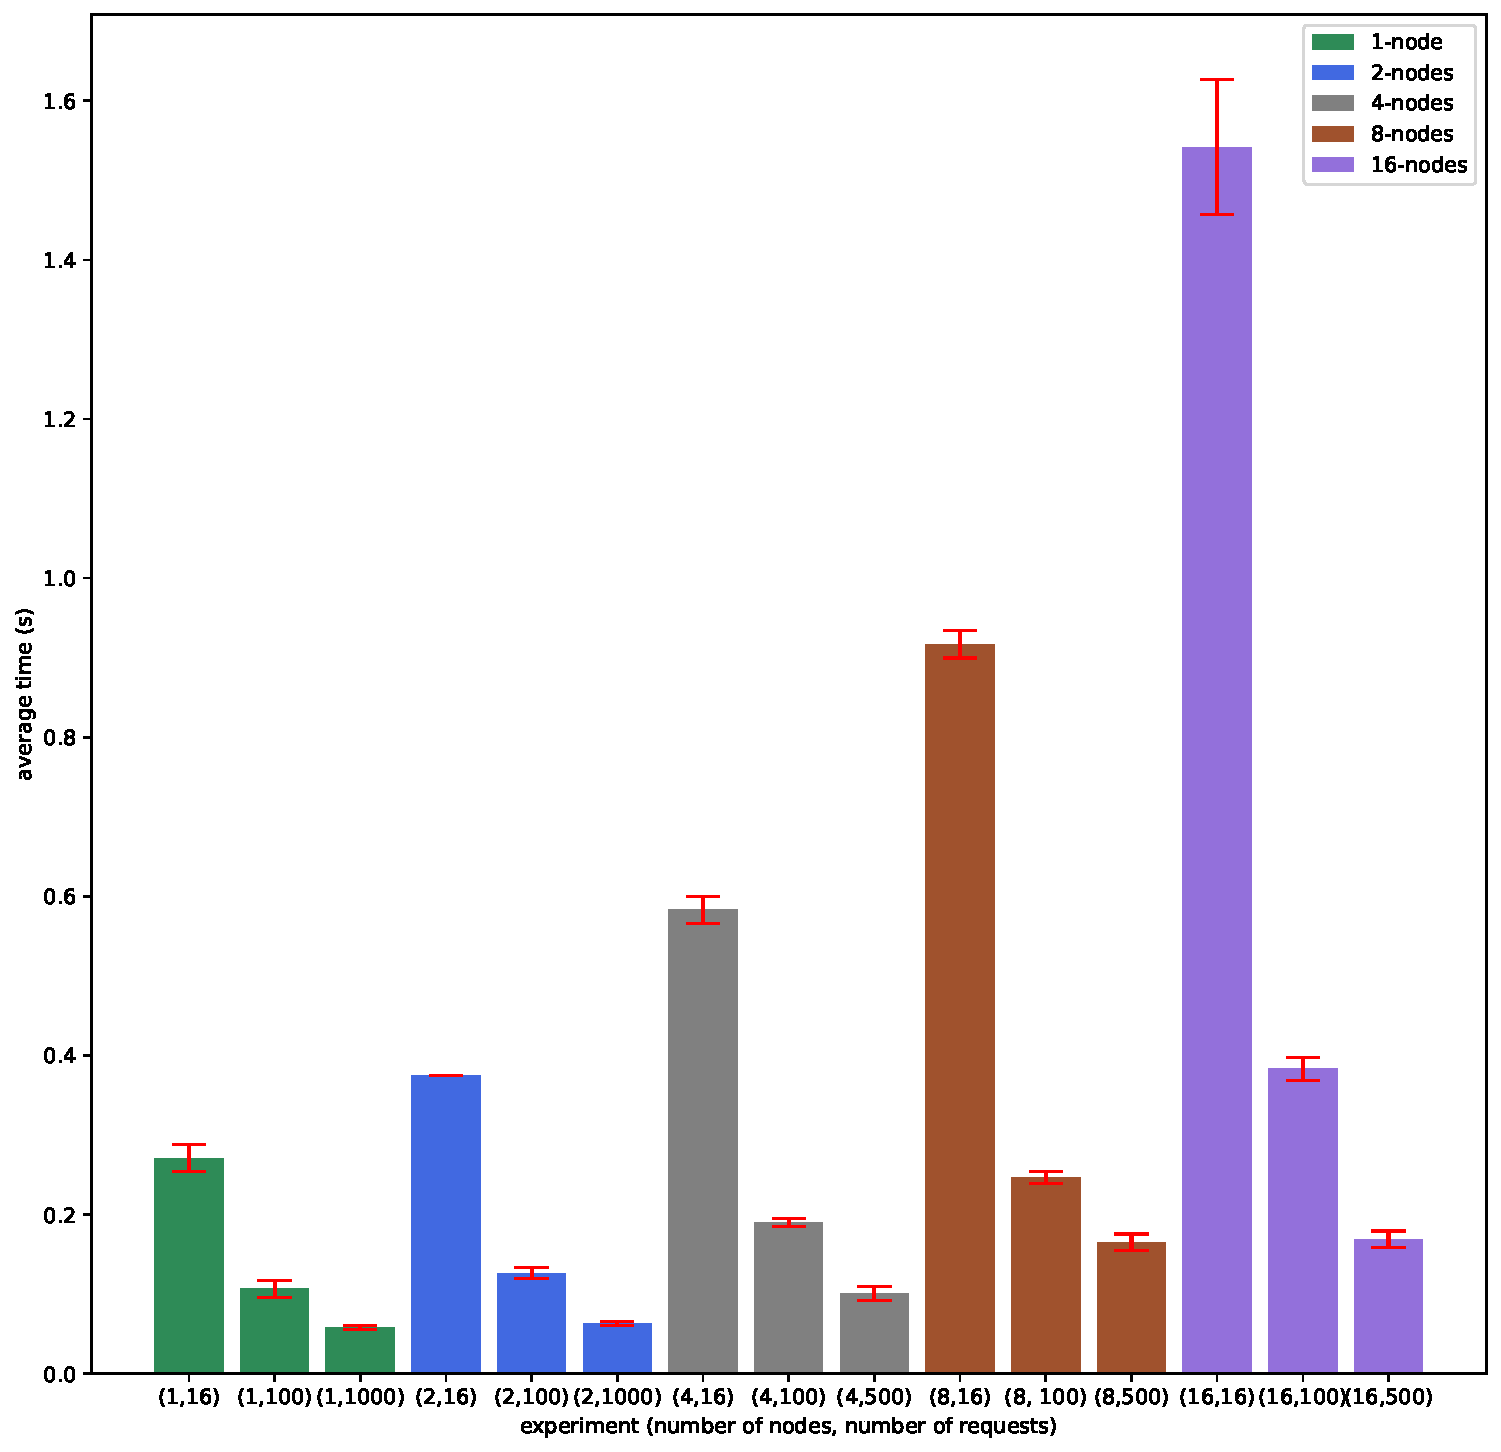
\includegraphics[width=7.5cm, height=5cm]{get.pdf}
	\caption{Histogram of average times for GET requests with different parameters}
\end{figure}

\setlength{\intextsep}{5pt plus 2pt minus 0pt}
\begin{figure}[!ht]
	\centering
	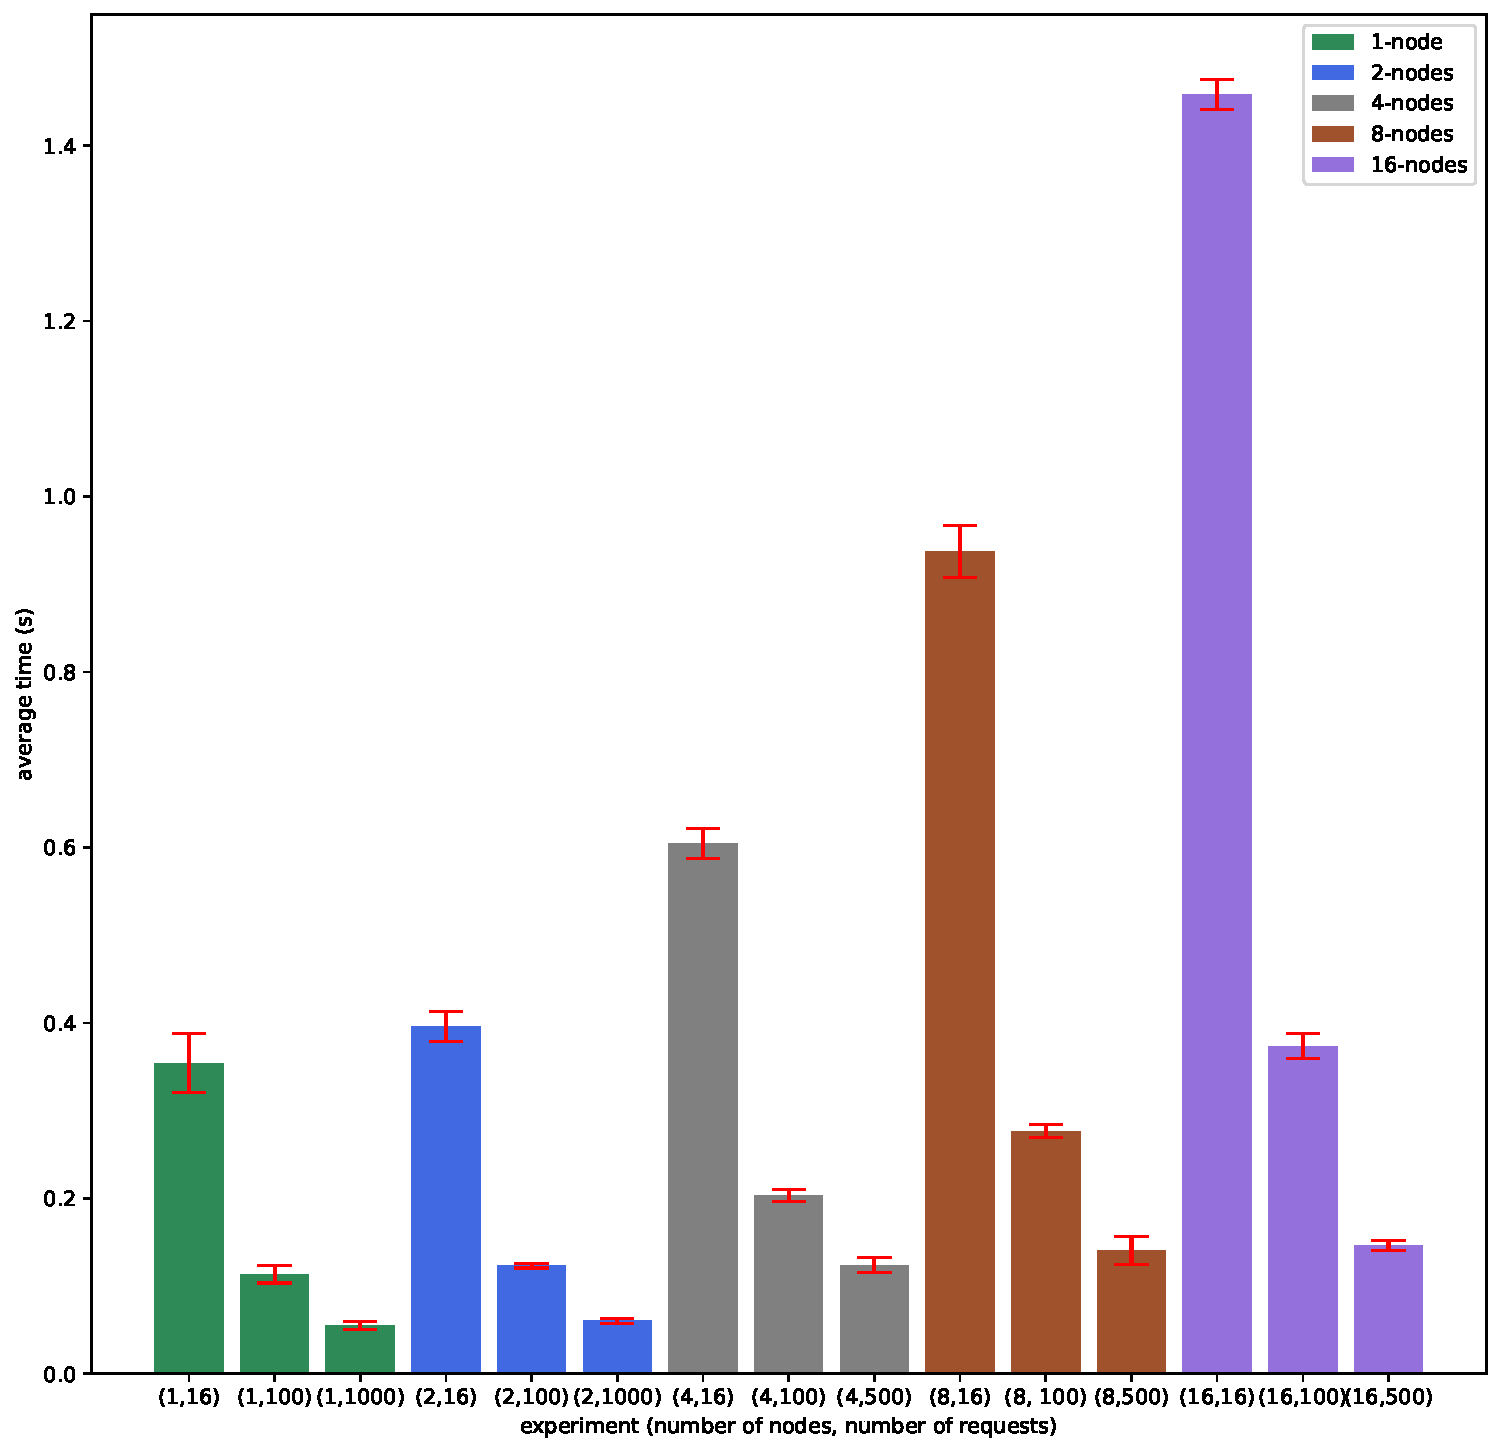
\includegraphics[width=7.5cm, height=5cm]{put.pdf}
	\caption{Histogram of average times for PUT requests with different parameters}
\end{figure}

Line graphs in Figure 4 and 5 were constructed for more precise interpretation and comparison of experiment results.\\

\setlength{\intextsep}{7pt plus 2pt minus 0pt}
\begin{figure}[!ht]
	\centering
	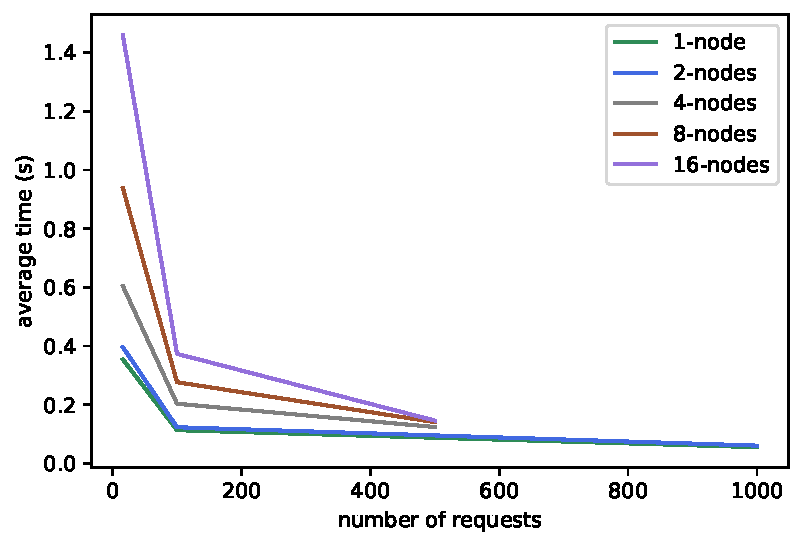
\includegraphics[width=7.5cm, height=5cm]{put_line.pdf}
	\caption{Line graph of average times for PUT requests with different parameters}
\end{figure}

\setlength{\intextsep}{5pt plus 2pt minus 0pt}
\begin{figure}[!ht]
	\centering
	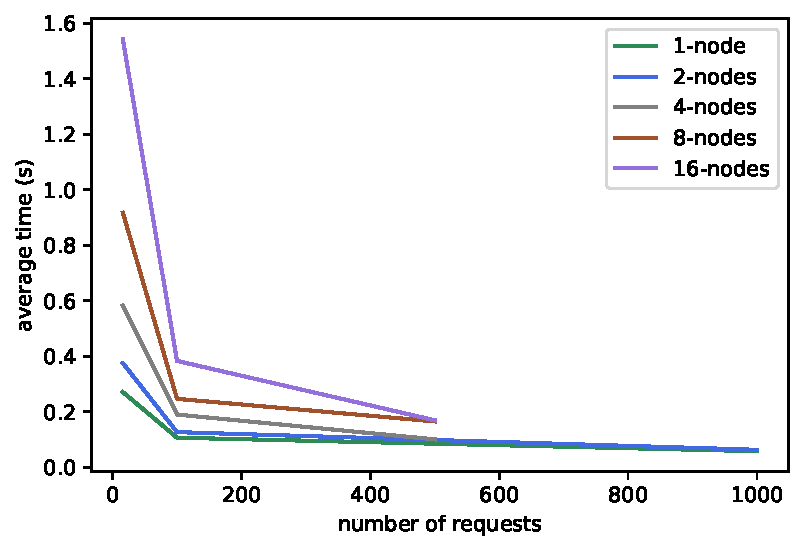
\includegraphics[width=7.5cm, height=5cm]{get_line.pdf}
	\caption{Line graph of average times for GET requests with different parameters}
\end{figure}

By observing these charts, it is obvious that response times increase with number of nodes in the network for a particular batch of requests and can this be explained by the rise in redundant HTTP calls among nodes when a network expands. However, this increasing factor seems to be diminishing when the size of the request batch increases. \\

Furthermore, for a given network with a fixed number of nodes, latency decreases as opposed to number of requests in the batch. A possible reason for this observation could be that the capability of a node to process query requests asynchronously while the rest are still in progress or being circulated in the network and thus maximizing the throughput relatively.\\

This entire behaviour is consistent across both request types (GET and PUT) despite the minor variations in latency. Lower average times are highly possible if the communication among nodes can be replaced with a better approach.

\section{Conclusion}

Finally, it can be concluded that the implemented key-value store is more appropriate when the number of queries is higher in terms of the performance for a given network of nodes. In contrast, number of nodes in the network has a negative impact on the query latency. \\ 

Thus, the distributed key-value store should be designed with a preferable number of nodes such that it addresses the trade-off between performance and other quantitative/non-quantitative measures of a distributed system (scalability, accessibility, load of queries, fault tolerance etc.) depending on the requirements of a given scenario.

\begin{thebibliography}{9}	
	\bibitem{chord}
	Ion Stoica, Robert Morris, David Karger, M. Frans Kaashoek, Hari Balakrishnan (2001) \emph{Chord: A Scalable Peer-to-Peer Lookup Service for Internet Applications }, MIT Laboratory for Computer Science.
	
	\bibitem{error}
	Lee, Dong and In, Junyong and Lee, Sangseok (2015) \emph{Standard deviation and standard error of the mean}, Korean journal of anesthesiology.
\end{thebibliography}

\appendix
\section{Source Code}
\href{https://github.com/YasiruR/dht/tree/master}{Github repository}

\end{document}
